\documentclass{article}
\usepackage{graphicx}
\usepackage{amsmath}
\usepackage{listings}
\usepackage{xcolor}
\usepackage{hyperref}
\usepackage{listings}
\usepackage{fancyhdr}
\usepackage[a4paper, hmargin = 1.5cm, head = 4cm, bottom = 2cm]{geometry}
\usepackage{amssymb}


\pagestyle{fancy}
\lhead{\includegraphics[width=0.27\textwidth]{assets/eth_logo.pdf}}
\rhead{Wahrscheinlichkeit und Statistik}
\lfoot{Spring Semester 2023}
\rfoot{\thepage}
\cfoot{}
\renewcommand{\footrulewidth}{1pt}

\begin{document}

\begin{titlepage}
    \thispagestyle{fancy}
    \renewcommand{\headrulewidth}{1pt}

    \center
    \vspace*{1.0cm}
    \Large Wahrscheinlichkeit und Statistik \\[.5 cm]
    \large
    \normalsize
    Gnkgo, Informatik B. Sc. 4. Semester \\
    \vfill
\end{titlepage}



\tableofcontents
\newpage

\section{Wichtig zu merken}

Wir haben eine $\sigma$-Algebra auf $\Omega$. Dann muss die leere, die volle und immer das jeweilige Komplement in der Algebra vorhanden sein.

\begin{figure}[h]m
    \centering
    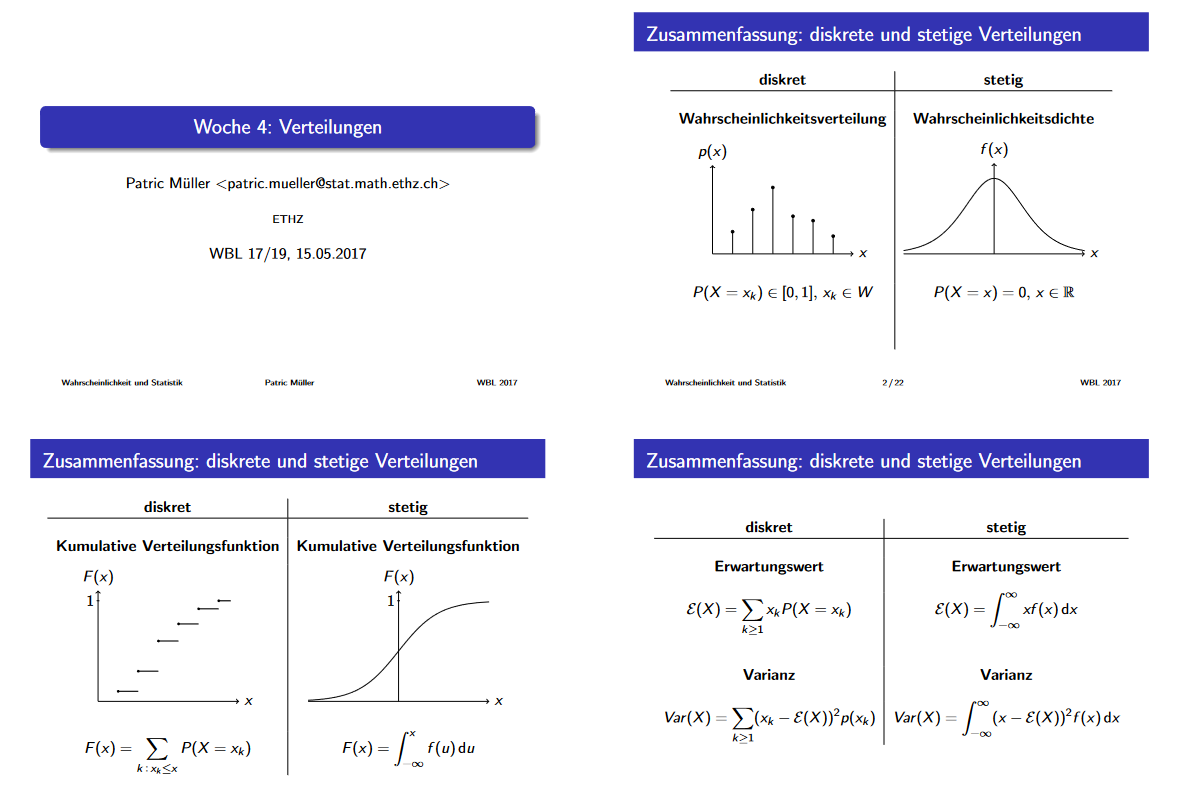
\includegraphics[width=0.7\linewidth]{Source/assets/diskrete_stetige_verteilung.png}
    \caption{Diskrete und stetige Verteilung}
\end{figure}

\section{Dichte}
\begin{itemize}
    \item Eine Wahrscheinlichkeitsdichte muss integriert über den gesamten Definitionsbereich 1 ergeben.
    \item Nichtnegativität: Die Dichte $f(x, y)$ muss für alle $x$ und $y$ größer oder gleich 0 sein.
    \item Seien $X$ und $Y$ zwei stetige Zufallsvariablen mit Dichte $f_X$ resp $f_Y$
    \begin{itemize}
        \item Nicht notwendigerweise gemeinsame Dichte
        \item Wenn $X$, $Y$ unabhängig, dann gemeinsame Dichte
        $$f_{X, Y}(x, y) = f_X(x) \cdot f_Y(y)$$
    \end{itemize}
\end{itemize}

\section{Wahrscheinlichkeiten}

\subsection{Approximationen}
\begin{itemize}
    \item Wenn $\text{Bin}()$ Wahrscheinlichkeit $p = \sim \frac{1}{2}$ hat, dann ist es wie eine Normalverteilung:
    $$X \stackrel{\text{approx.}}{\sim} \mathcal{N}\left(\frac{n}{2}, \frac{n}{4}\right)$$
    \item Wenn $\text{Bin}()$ Wahrscheinlichkeit $p$ sehr klein hat und $n$ sehr groß, dann ist es wie eine Poissonverteilung:
    $$X \stackrel{\text{approx.}}{\sim} \text{Poi}(\lambda = np)$$
\end{itemize}

\section{Quiz}
Sei $(\Omega, F, P)$ ein Wahrscheinlichkeitsraum und $A \in F$. Was ist korrekt:
\begin{itemize}
    \item $A$ ist unabhängig von sich selbst genau dann, wenn $P[A] = 1$.
    \item Nach Definition ist $A$ unabhängig von sich selbst genau dann, wenn $P[A \cap A] = P[A] \cdot P[A]$, also genau für $P[A] = (P[A])^2$ wegen $A \cap A = A$. Wegen $P[A] \geq 0$ ist die letzte Bedingung aber äquivalent zu $P[A] \in \{0, 1\}$.
\end{itemize}

Sei $p \in [0, 1]$, sei $X$ eine $\text{Ber}(p)$-verteilte Zufallsvariable und definiere $Z := (2X - 1)^2$. Was ist der Erwartungswert $E[Z]$?
\begin{itemize}
    \item Da $X$ Werte in $\{0, 1\}$ annimmt, nimmt $Z$ Werte in $\{1\}$ an. Somit gilt $E[Z] = 1 \cdot P[Z = 1] = 1$.
\end{itemize}

Es gilt: $P[X \geq 1|X \leq 1] = P[X = 1] P[X = 0] + P[X = 1] = \frac{\lambda \cdot e^{-\lambda}}{e^{-\lambda} + \lambda \cdot e^{-\lambda}} = \frac{\lambda}{1 + \lambda}$

Seien $X$ und $Y$ zwei diskrete Zufallsvariablen mit gemeinsamer Gewichtsfunktion $p_{X,Y}$
\begin{itemize}
    \item $E[XY] = \sum_{x \in W_X} \sum_{y \in W_Y} x \cdot y \cdot p_{X, Y}(x, y)$
\end{itemize}

Stetige Zufallsvariable
\begin{itemize}
    \item Die Verteilungsfunktion ist stetig.
    \item Dichtefunktion kann auch einmal (strikt) größer als 1 sein.
\end{itemize}

Seien $X$ und $Y$ zwei Zufallsvariablen mit gemeinsamer Dichte $f_{X, Y}$.
\begin{itemize}
    \item Die Zufallsvariablen $X$ und $Y$ sind immer stetig.
\end{itemize}

\section{Errors}

\begin{tabular}{|c|c|c|}
    \hline
    & $H_0$ True & $H_0$ False \\
    \hline
    Reject $H_0$ & Type I Error & $\checkmark$ \\
    \hline
    Fail to reject $H_0$ & $\checkmark$ & Type II Error \\
    \hline
\end{tabular}

\textbf{Type I error:} Null Hypothese verwerfen, obwohl sie wahr ist.

\textbf{Type II error:} Null Hypothese nicht verwerfen, obwohl sie falsch ist. 

$$P(\text{type I error } / H_0 \text{ is true}) = \alpha$$
$$P(\text{type II error } / H_0 \text{ is false}) = \beta$$
$$P(\text{rejecting a false } H_0) = 1 - \beta$$

\end{document}
